\newcommand{\FigAntiprotonEndpoint}{
\begin{figure}[btp]
\centering
\subfloat[][\figlabel{bg:antiprotons:end-point:tungsten}Tungsten]{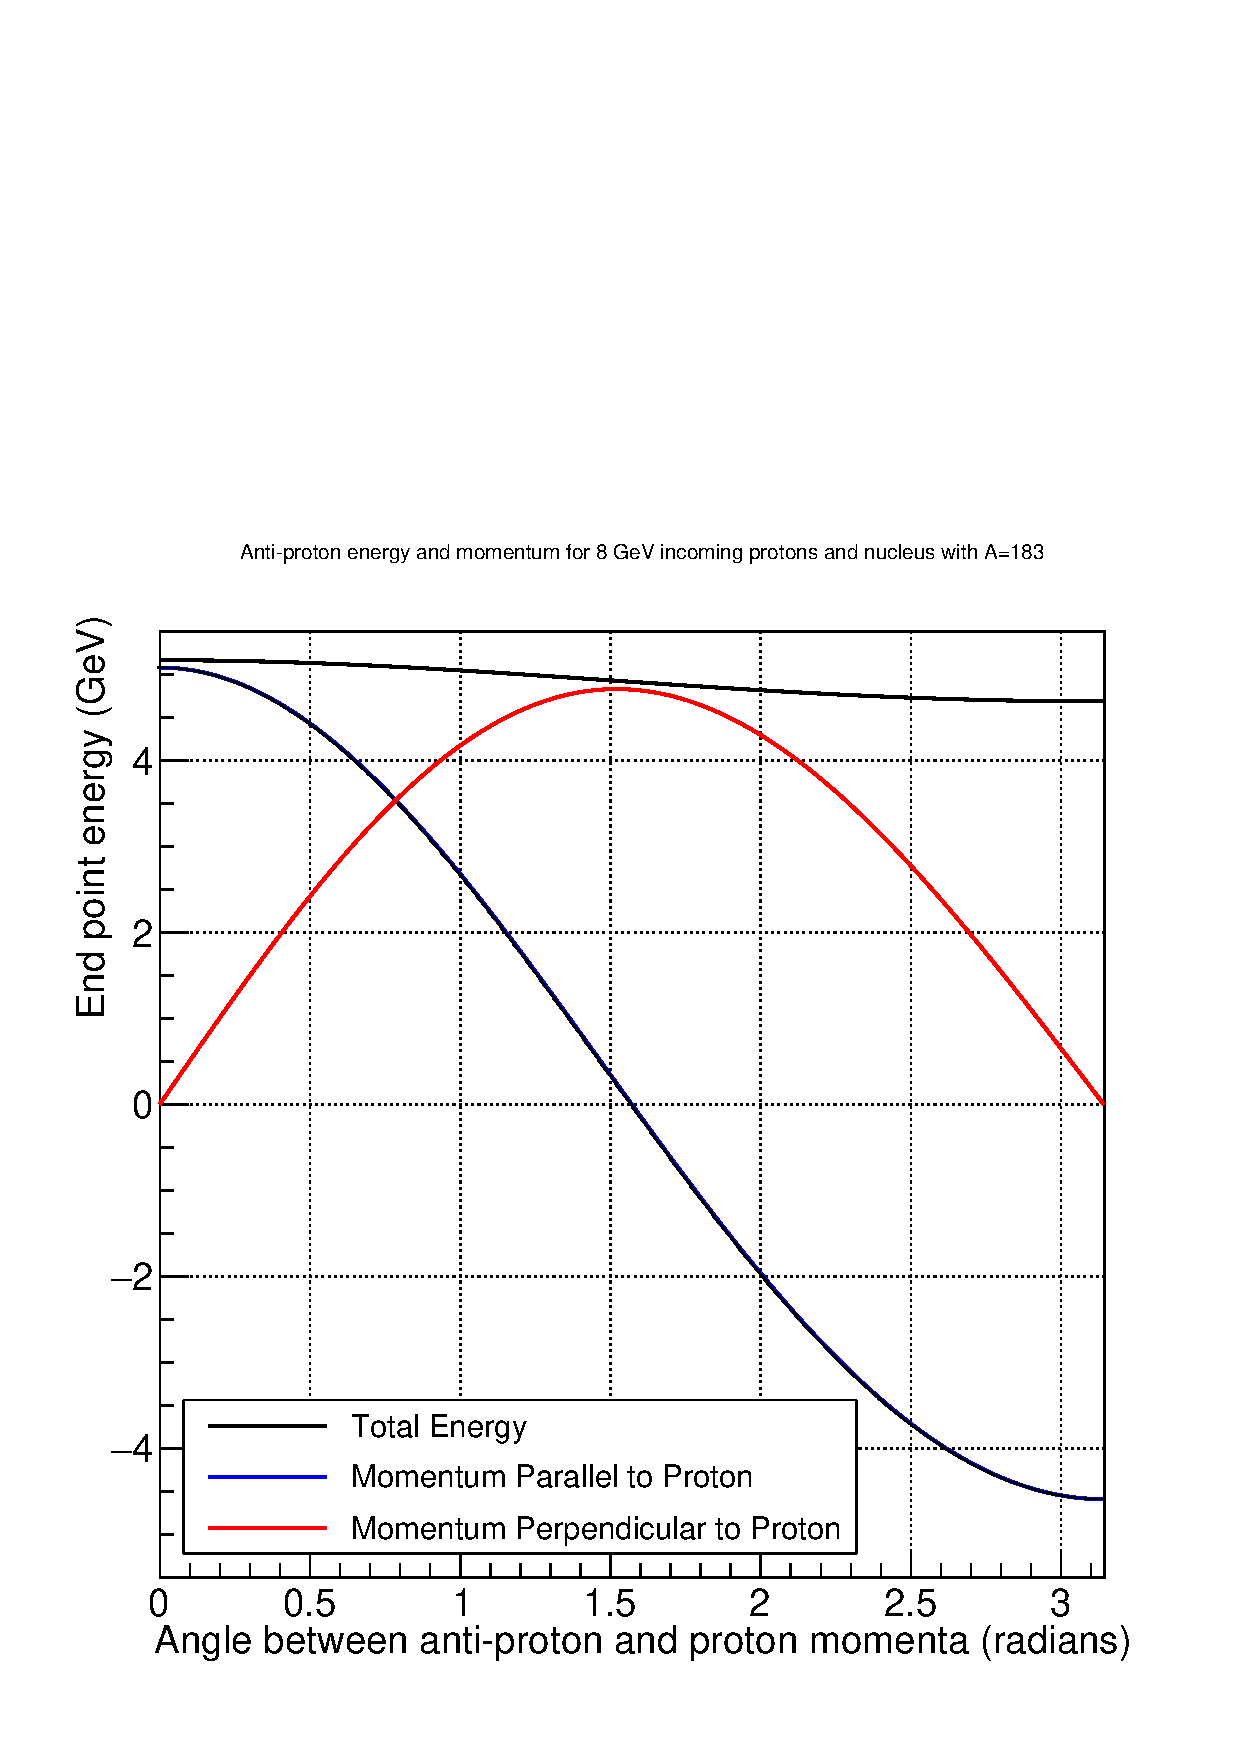
\includegraphics[width=0.49\textwidth,clip=true,trim=0 0 1cm 2cm]{figs/backgrounds/Antiproton_Tungsten_theta_lab.pdf}}%\hspace{0.5cm}%
\subfloat[][\figlabel{bg:antiprotons:end-point:carbon}Carbon    ]{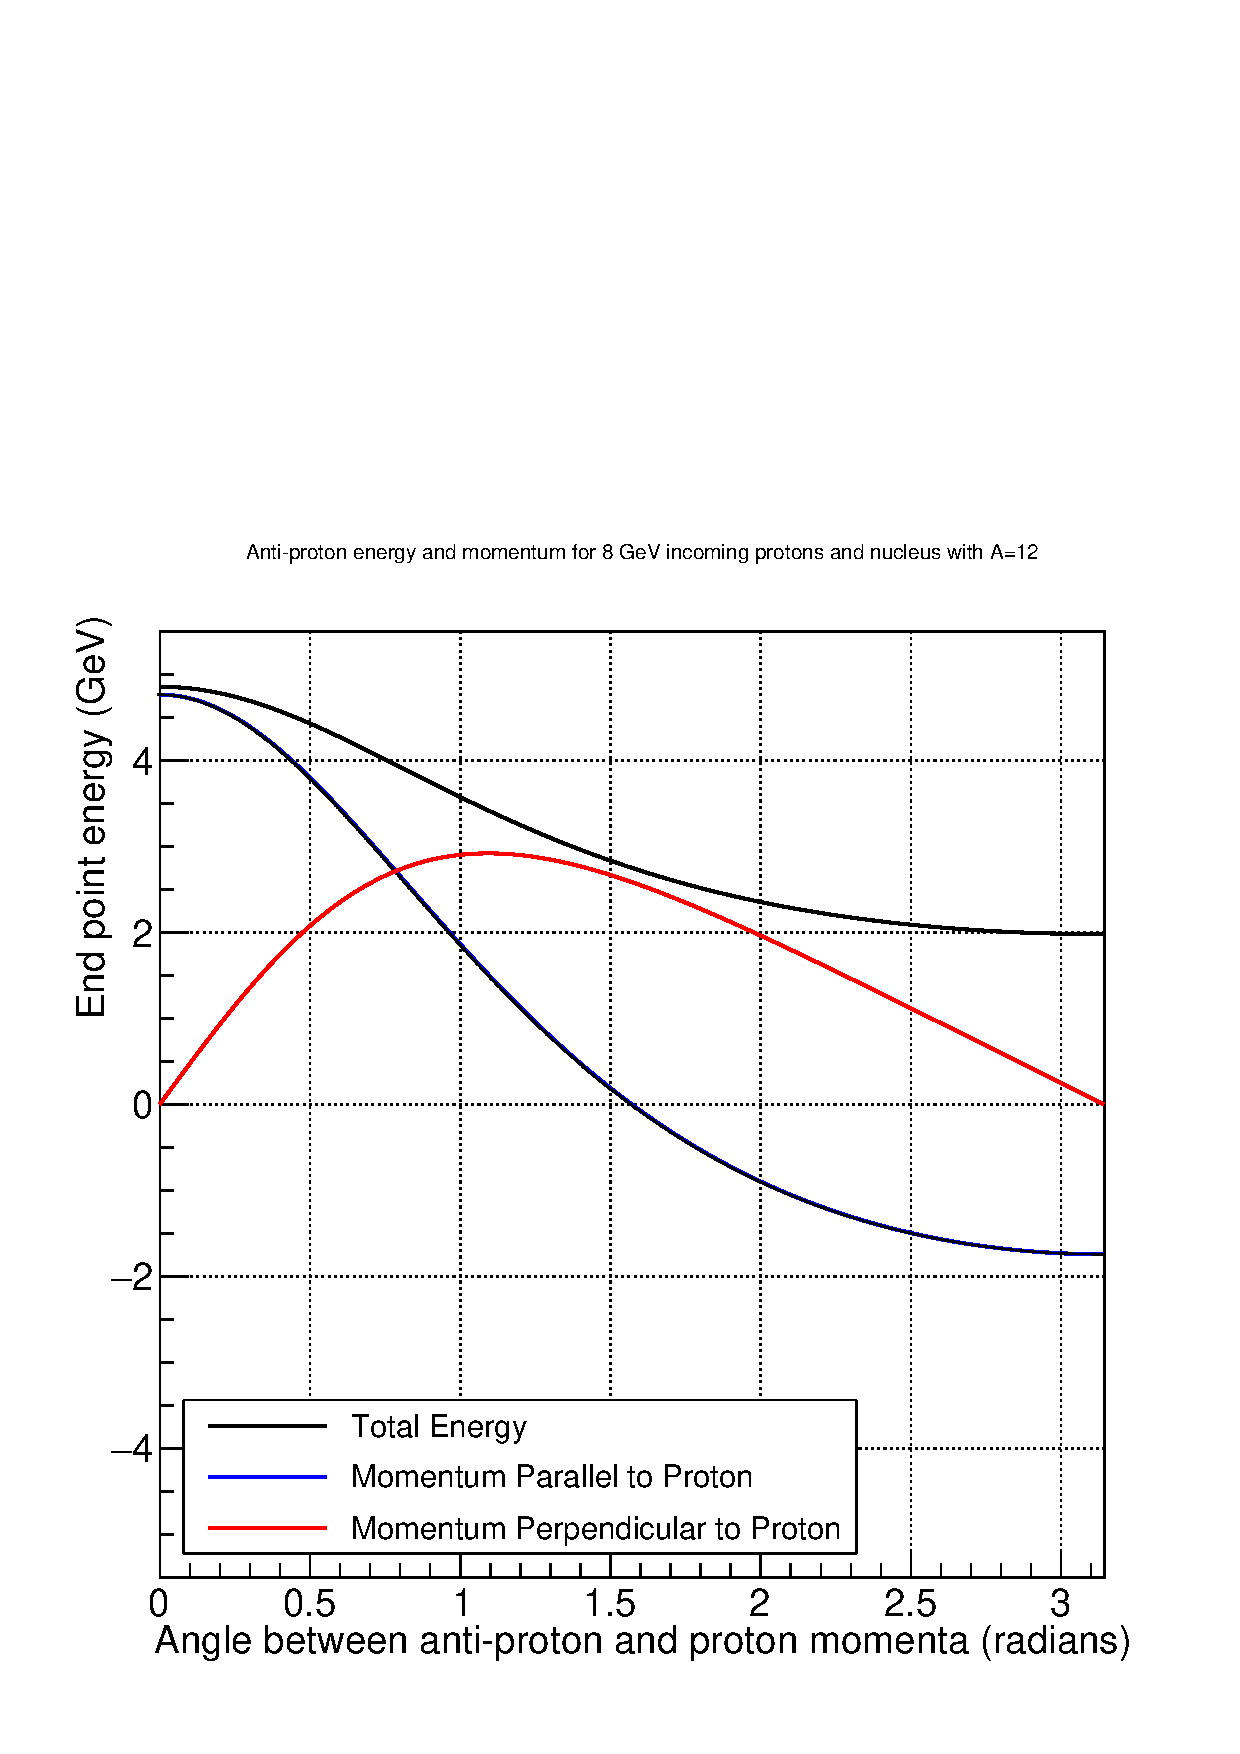
\includegraphics[width=0.49\textwidth,clip=true,trim=0 0 1cm 2cm]{figs/backgrounds/Antiproton_Carbon_theta_lab}}
\caption{\figlabel{bg:antiprotons:end-point}
The kinematic end-point for antiproton production as a function of the out-going antiproton direction with respect to the incoming proton in the frame of the target nucleus (the lab frame).
The absolute end-point is only achieved when the nucleus and out-going protons recoils coherently.
}
\end{figure}
}

\newcommand{\FigAntiprotonFits}{
\begin{figure}[tbp]
\centering
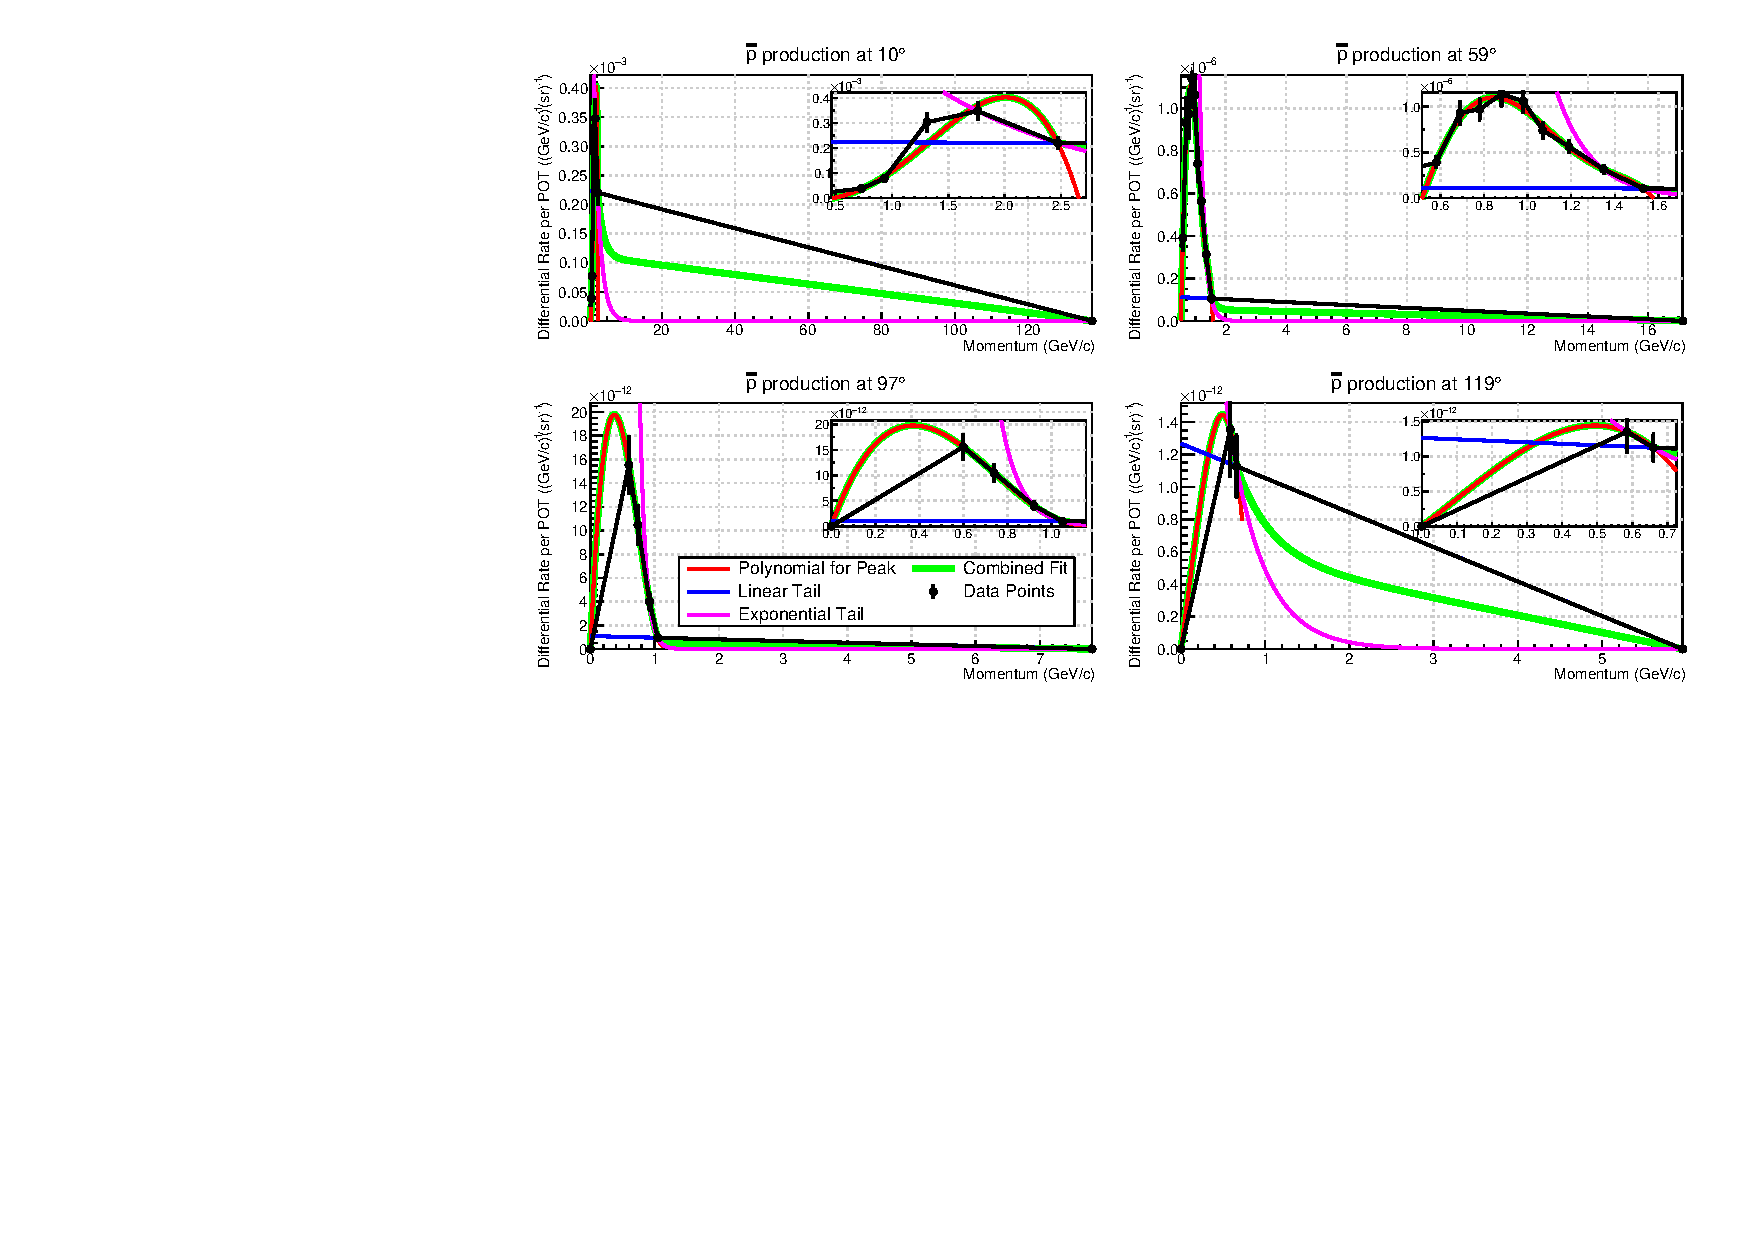
\includegraphics[width=1.0\textwidth,trim=0 0 0.45cm 0,clip]{figs/backgrounds/AntiprotonFits.pdf}
\caption{\figlabel{bg:antiprotons:fits}
Piecewise fitting to experimental data and kinematic end-points.
Inlays show a zoom around the experimental data points.
}
\end{figure}
}

\newcommand{\FigAntiprotonAngularDependence}{
\begin{figure}[tbp]
\centering
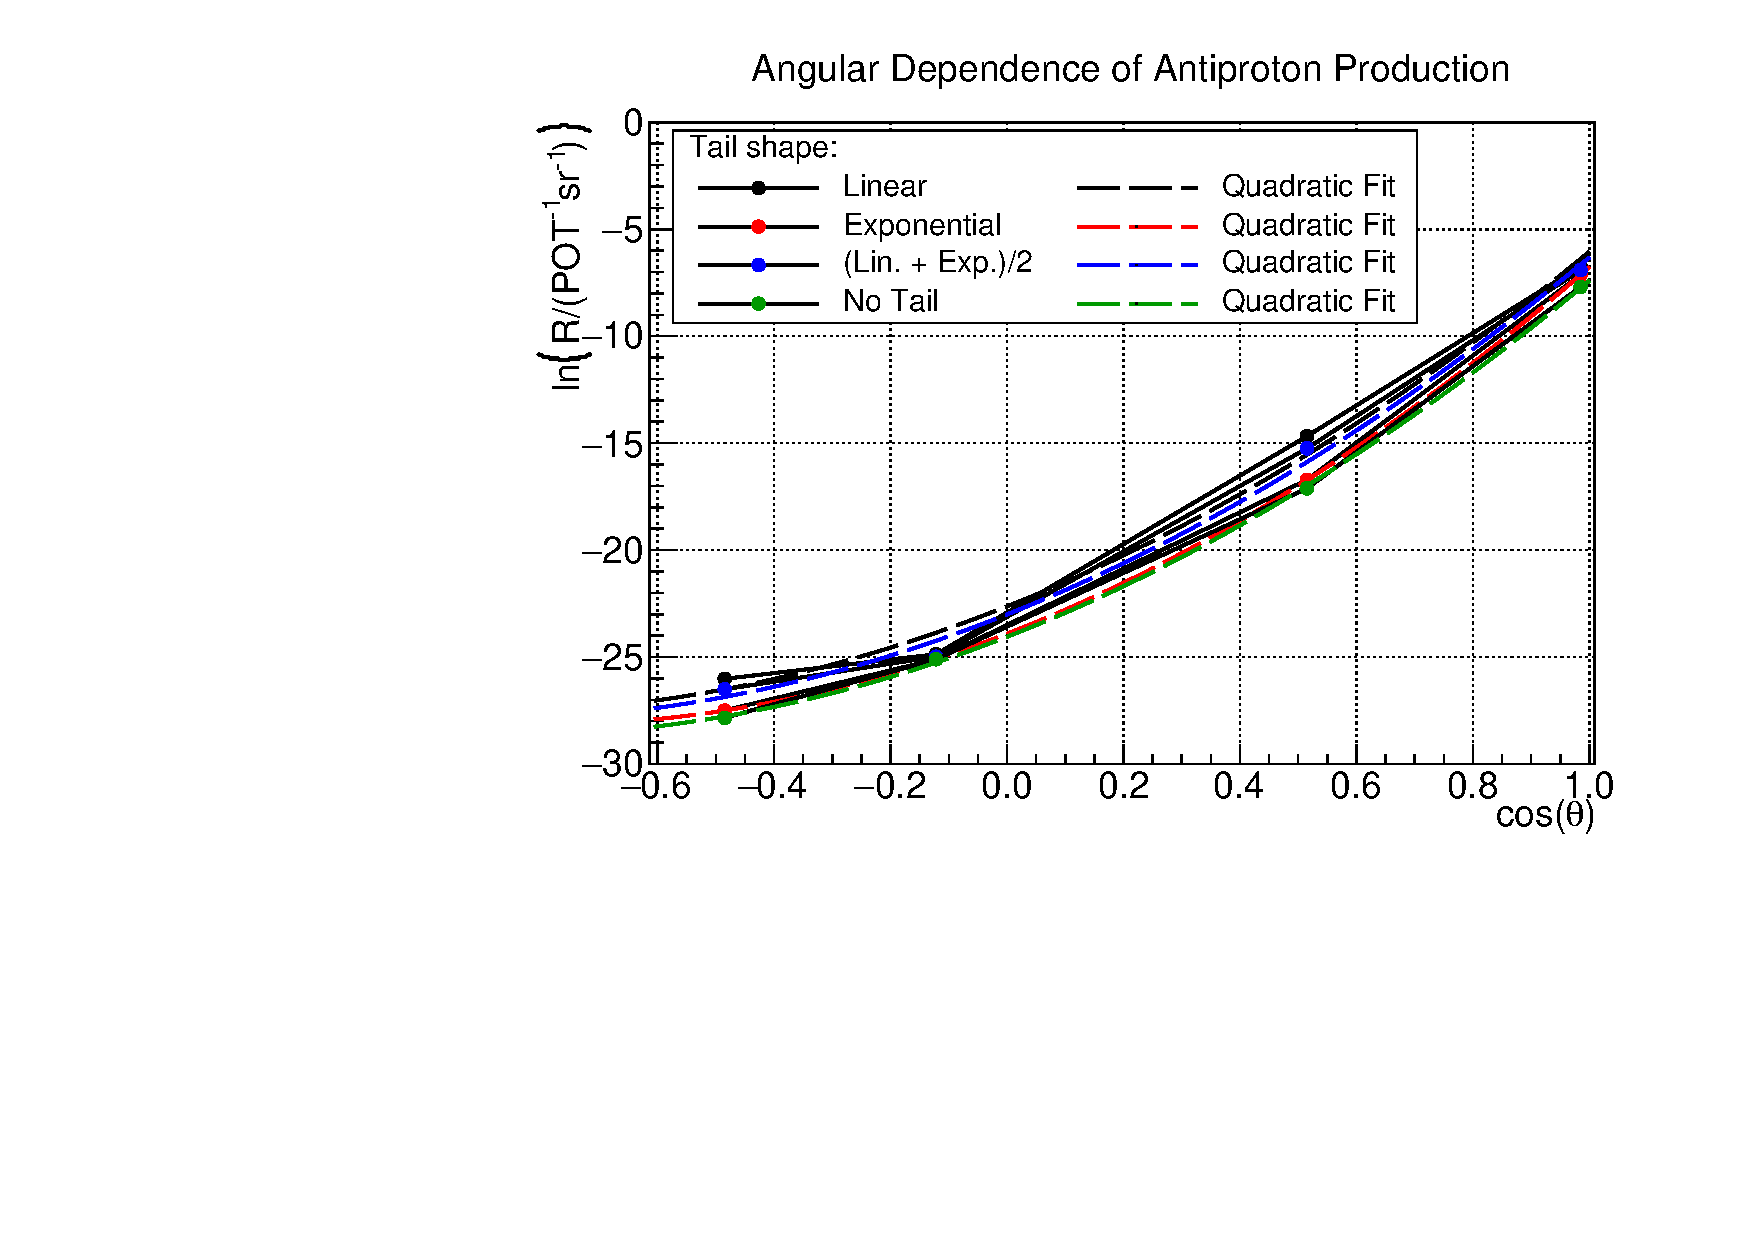
\includegraphics[width=0.8\textwidth,trim=0 0 1.4cm 1cm,clip]{figs/backgrounds/AntiprotonAngularDependence.pdf}
\caption{\figlabel{bg:antiprotons:angular}
The angular dependence of the rate of antiproton emission, integrated over all momenta.
The different lines represent the different fits to the high momentum part of the spectrum.
The relationship given in~\cite{Boyarinov:1994tp} would suggest the data here should fit a straight line.
The dashed lines represent instead a quadratic fit to these points, which looks like a better fit.
For reweighting events the interpolated (straight solid) lines were used to be conservative.
}
\end{figure}
}

\newcommand{\TabAntiprotonRegions}{
\begin{table}[bp]
\centering
	\begin{tabular}{rccl}
		Region & Data source & Fitted Momentum Function & Total $\bar{p}$ per POT \\
\hline
                $0 \le \theta< 59\degree$ & 10\degree \cite{Kiselev:2012sj} &         & $5.32\times10^{-4}  $\\
                $59 \le \theta< 97\degree$ & 59\degree \cite{Kiselev:2012sj} &        & $2.80\times10^{-8 } $\\
                $97 \le \theta< 119\degree$ & 97\degree \cite{Boyarinov:1994tp} &     & $2.39\times10^{-12} $\\
                $119 \le \theta< 180\degree$ & 119\degree \cite{Boyarinov:1994tp} &   & $1.22\times10^{-12} $\\

\hline
\end{tabular}
\caption{\tablabel{bg:antiprotons:regions}
Regions and fits used to simulate antiproton production.  
The values in the final column are result of converting to rates per POT and integrating the differential cross-sections measured in \cite{Boyarinov:1994tp,Kiselev:2012sj}.
%integrated the fitted and extrapolated spectra and then integrates over the fitted angular dependence.
}
\end{table}
}

